%%%%%%%%%%%%%%%%%%%%%%%%%%%%%%%%%%%%%%%%%%%%%%%%%%%%%%%%%%%%%%%%%%%%%%%%%%%
%% This file is part of the book
%%
%% Algorithmic Graph Theory
%% http://code.google.com/p/graph-theory-algorithms-book/
%%
%% Copyright (C) 2009, 2010, 2011 Minh Van Nguyen <nguyenminh2@gmail.com>
%%
%% See the file COPYING for copying conditions.
%%%%%%%%%%%%%%%%%%%%%%%%%%%%%%%%%%%%%%%%%%%%%%%%%%%%%%%%%%%%%%%%%%%%%%%%%%%

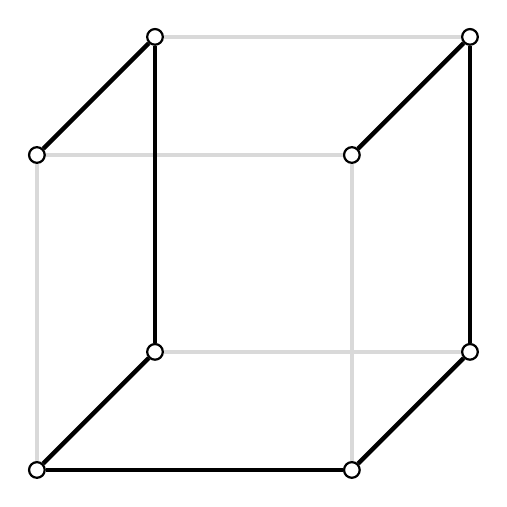
\begin{tikzpicture}
[nodedecorate/.style={shape=circle,inner sep=2pt,draw,thick},%
  darkline/.style={-,ultra thick},
  lightline/.style={-,ultra thick,color=gray!30}]
% nodes or vertices
% foreground square
\node (1) at (0,0) [nodedecorate] {};
\node (2) at (4,0) [nodedecorate] {};
\node (3) at (4,4) [nodedecorate] {};
\node (4) at (0,4) [nodedecorate] {};
% background square
\node (5) at (1.5,1.5) [nodedecorate] {};
\node (6) at (5.5,1.5) [nodedecorate] {};
\node (7) at (5.5,5.5) [nodedecorate] {};
\node (8) at (1.5,5.5) [nodedecorate] {};
% edges or lines
\path
% foreground square
(1) edge[darkline] node {} (2)
(2) edge[lightline] node {} (3)
(3) edge[lightline] node {} (4)
(4) edge[lightline] node {} (1)
% background square
(5) edge[lightline] node {} (6)
(6) edge[darkline] node {} (7)
(7) edge[lightline] node {} (8)
(8) edge[darkline] node {} (5)
% joining foreground and background squares
(1) edge[darkline] node {} (5)
(2) edge[darkline] node {} (6)
(3) edge[darkline] node {} (7)
(4) edge[darkline] node {} (8);
\end{tikzpicture}
